\chapter{Project Plan}

\instructions{
    Describe the project plan as covered in the SEP2 module. A project plan typically consists of the following topics:
    
    \begin{itemize}
        \item Processes, meetings and roles
        \item Phases, iterations and milestones
        \item A \textbf{rough} list of things to be done (work items)
        \item Risk management
        \item Planning Tools (issue tracker, time tracker, ...)
    \end{itemize}
    
    You should \textbf{\underline{not}} describe your \textbf{technical solution} in this chapter. It is all about organizing your project.
}

\section{Processes}
For the long-term planning we use RUP (\ref{phases}).
For the short-term planning we use Scrum.
The Scrum roles and other assignments are made in \ref{roles}.
The Scrum Events (Sprint Planning, Sprint Review, ...) are declared in \ref{meetings}.
The Gitlab Issue feature is used to model the Product Backlog and Sprint Backlog.

\section{Roles}
\label{roles}

\begin{tabular}{|l|l|}
    \textbf{Role} & \textbf{Person}\\
    \hline
    \textbf{Session Chair:} & changes every week \\
    \textbf{Product Owner (PO):} & The whole team \\
    \textbf{Developer:} & Benjamin Plattner, Olivier Lischer, Pascal Lehmann\\
    \textbf{Network:} & Jan Untersander, Petra Heeb \\
\end{tabular}
\newline
\noindent The classification in \textsl{Developer} and \textsl{Network} shows only the primary strengths.
Members of the \textsl{Developer} group sometimes also work on the network part and vice versa.


\section{Meetings}
\label{meetings}
We have two weekly meetings.
A team internal meeting on each Monday.
This meeting is used to implement:
\begin{itemize}
  \item Sprint Planning
  \item Sprint Retrospective 
\end{itemize}

\noindent The second meeting is on each Tuesday with the advisor Laurent Metzger.
In this meeting the \textsl{Sprint Review} is done.
The \textsl{Daily Scrum} take places during the week at lunch or during breaks.
One Sprint last between two and four weeks.


\section{Phases, iterations and milestones}
\label{phases}
In our project we work with the four project phases which are defined also in the RUD model which we used for our rough project plan. The four phases are:
\begin{itemize}
    \item Inception
    \item Elaboration
    \item Construction
    \item Transition
\end{itemize}

\subsection{Inception}
The first phase is the \textit{Inception} phase. In this phase we start the new project and use to define the following things to plan our project:
\begin{itemize}
    \item Approximate vision
    \item Defining the scope
    \item Rough estimates for efforts
\end{itemize}

\subsection{Elaboration}
The second phase is called \textit{Elaboration}. This phase is used to start the practical part of the project and the goal of this phase is to eliminate potential risks. There are some parts you need to handle in this phase:
\begin{itemize}
    \item Identification of most requirements
    \item Iterative implementation of core architecture
    \item Resolution of high risks
    \item More realistic estimates for efforts
\end{itemize}

\subsection{Construction}
The third and biggest phase is the \textit{Construction} phase. In this phase the team need to make the project around the risk parts of the project. In this phase the risk parts should be already solved.
The contents of this phase are:
\begin{itemize}
    \item Iterative implementation of functionality
    \item Resolution of lower risks
    \item Preparation for deployment
\end{itemize}

\subsection{Transition}
The last project phase is to finish the project and to test the project with the whole environment and called \textit{Transition} phase.
The basic points of this finish phase are:
\begin{itemize}
    \item Beta Tests
    \item Deployment
    \item Tie up any loose ends
\end{itemize}

\section{Project Plan}
\subsection{RUD - Rational Unified Process}
To define a rough project plan we use the RUD model. \newline
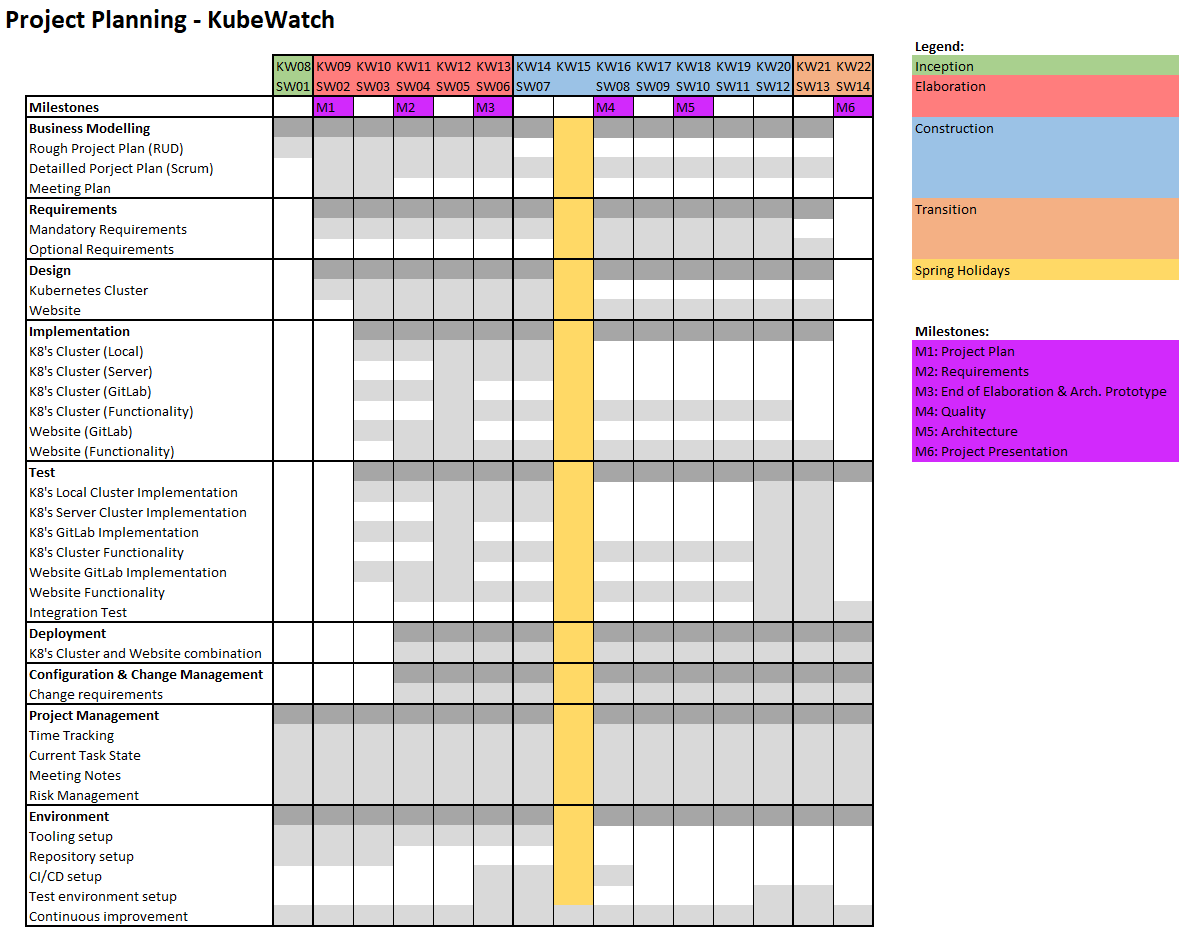
\includegraphics[height=10cm]{resources/project-plan-RUD.png}

\subsection{Scrum}
For the short term planning iteration we use the Scrum method.

\section{Risk management}


\section{Planning Tools}
For planning our work, for issue handling and time tracking we use the GitLab tool which is hosted by the OST themself.